\section{ÔN TẬP CHƯƠNG 1}
\subsection{TRẮC NGHIỆM NHIỀU PHƯƠNG ÁN LỰA CHỌN}
\setcounter{ex}{0}
\Opensolutionfile{ans}[ans/FINAL-CHAPTER1-TN]
\begin{ex}
Lĩnh vực nghiên cứu nào sau đây là của Vật lí?	\choice
	{Nghiên cứu về sự thay đổi của các chất khi kết hợp với nhau} 
	{\True Nghiên cứu về các dạng chuyển động và các dạng năng lượng khác nhau}
	{Nghiên cứu sự phát minh và phát triển của các vi khuẩn}
	{Nghiên cứu về sự hình thành và phát triển của các tầng lớp, giai cấp trong xã hội}
	\loigiai {Lĩnh vực nghiên cứu của Vật lí là nghiên cứu về các dạng chuyển động và các dạng năng lượng khác nhau.}
\end{ex}

\begin{ex}
Biểu hiện nào sau đây \textbf{không} phải là biểu hiện của phát triển năng lực Vật lí?	\choice
	{Có được kiến thức kỹ năng cơ bản về Vật lí}
	{Vận dụng được kiến thức, kĩ năng để khám phá, giải quyết các vấn đề có liên quan trong học tập cũng như trong cuộc sống}
	{Nhận biết được năng lực, sở trường của bản thân, định hướng nghề nghiệp}
	{\True Nhận biết được hạn chế của bản thân để tìm cách khắc phục}
	
	\loigiai{Nhận biết được hạn chế của bản thân để tìm cách khắc phục.}
\end{ex}

\begin{ex}
Cấp độ vi mô là gì?	\choice
	{\True Cấp độ dùng để mô phỏng vật chất bé nhỏ}
	{Cấp độ to, nhỏ phụ thuộc vào qui mô khảo sát}
	{cấp độ mô phỏng tầm rộng lớn hay rất lớn của vật chất}
	{Cấp độ tinh vi khi khảo sát một hiện tượng Vật lí}
	
	\loigiai{Cấp độ vi mô dùng để mô phỏng các vật chất bé nhỏ.}	
\end{ex}


\begin{ex}
	Đặc trưng của cuộc cách mạng công nghiệp lần thứ nhất là \choice
	{\True Thay thế sức lực cơ bắp bằng máy móc}
	{Sử dụng các thiết bị điện trong mọi lĩnh vực của đời sống}
	{Tự động hóa các quá trình sản xuất}
	{Sử dụng trí tuệ nhân tạo, robot và internet toàn cầu}
	\loigiai {Đặc trưng của cuộc cách mạng công nghiệp lần thứ nhất là thay thế sức lực cơ bắp bằng máy móc.}
\end{ex}


\begin{ex}
	Các nhà triết học tìm hiểu thế giới tự nhiên dựa trên quan sát và suy luận chủ quan thể hiện ở nội dung nào sau đây?\choice
	{\True Vật nặng bao giờ cũng rơi nhanh hơn vật nhẹ}
	{Hiện tượng ánh sáng làm bật các electron ra khỏi kim loại}
	{Cái lông chim và hòn bi rơi nhanh như nhau trong ống hút hết không khí}
	{Hiện tượng cầu vồng}
	\loigiai {Vật nặng bao giờ cũng rơi nhanh hơn vật nhẹ.}
\end{ex}


\begin{ex}
	Ý nào dưới đây \textbf{không} phải là vai trò của khoa học tự nhiên trong đời sống?\choice
	{Mở rộng sản xuất, phát triển kinh tế.}
	{Bảo vệ môi trường, ứng phó với biển đổi khí hậu}
	{Bảo vệ sức khỏe và cuộc sống của con người}
	{\True Định hướng tư tưởng, phát triển hệ thống chính trị}
	\loigiai {Định hướng tư tưởng, phát triển hệ thống chính trị không phải là vai trò của khoa học tự nhiên trong đời sống. }
\end{ex}

\begin{ex}
	Thiết bị nào sau đây có ứng dụng kiến thức về nhiệt là chủ yếu?\choice
	{Điện thoại}
	{\True Nhiệt kế}
	{Cân điện tử}
	{Ti vi}
	\loigiai {Thiết bị ứng dụng kiến thức chủ yếu về nhiệt là nhiệt kế.}
\end{ex}

\begin{ex}
	Kiến thức về từ trường Trái Đất được dùng để giải thích đặc điểm nào của loài chim di trú? \choice
	{\True Xác định hướng bay}
	{Làm tổ}
	{Sinh sản}
	{KiếM ăn}
	\loigiai {Kiến thức về từ trường Trái Đất được dùng để giải thích đặc điểm xác định hướng bay của loài chim di trú.}
\end{ex}

\begin{ex} 
Cho các dữ kiện sau.\vspace{-1cm}
\begin{center}
	\begin{tabular}{L{7cm}L{7cm}L{7cm}}
		\textbf{1.} Kiểm tra giả thuyết.&\textbf{2.} Hình thành giả thuyết.&\textbf{3.} Rút ra kết luận.\\
		\textbf{4.} Đề xuất vấn đề.& \textbf{5.} Quan sát hiện tượng, suy luận.
	\end{tabular}
\end{center}
\vspace{-0.5cm}
Sắp xếp lại đúng các bước tìm hiểu thế giới tự nhiên dưới góc độ vật lí. \choice
	{1 – 2 – 3 – 4 – 5}
	{2 – 1 – 5 – 4 – 3}
	{5 – 2 – 1 – 4 – 3}
	{\True 5 – 4 – 2 – 1 – 3}
	\loigiai {Thứ tự đúng của các bước tìm hiểu thế giới tự nhiên dưới góc độ Vật lí là \\
		Quan sát hiện tượng, suy luận;
		Đề xuất vấn đề;
		Hình thành giả thuyết;
		Kiểm tra giả thuyết;
		Rút ra kết luận.}
\end{ex}

\begin{ex} 
	Các hiện tượng vật lí nào sau đây liên quan đến phương pháp thực nghiệm.\choice
	{Ô tô khi chạy đường dài có thể xem ô tô như là một chất điểm}
	{\True Thả rơi một vật từ trên cao xuống mặt đất}
	{Quả địa cầu là mô hình thu nhỏ của Trái Đất}
	{Để biểu diễn đường truyền của ánh sáng người ta dùng tia sáng}
	\loigiai {Thả rơi một vật từ trên cao xuống mặt đất.}
\end{ex}

\begin{ex} 
	Khi gặp sự cố mất an toàn trong phòng thực hành, học sinh cần \choice
	{\True báo cáo ngay với giáo viên trong phòng thực hành}
	{tự xử lí và không báo với giáo viên}
	{nhờ bạn xử lí sự cố}
	{tiếp tục làm thí nghiệm}
	\loigiai {Khi gặp sự cố mất an toàn trong phòng thực hành, học sinh cần báo cáo ngay với giáo viên trong phòng thực hành.}
\end{ex}

\begin{ex} 
	Khi phòng thực hành xuất hiện cháy thì ta cần phải \choice
	{\True ngắt điện, di chuyển các chất dễ cháy ra ngoài và chống cháy lan, cứu người, cứu tài sản, dập tắt đám cháy}
	{chạy ra khỏi phòng, đi tìm thêm người đến dập đám cháy}
	{nngắt nguồn điện, dùng nước dập đám cháy}
	{dùng nước dập đám cháy}
	\loigiai {Khi phòng thực hành xuất hiện cháy thì ta cần phải ngắt điện, di chuyển các chất dễ cháy ra ngoài và chống cháy lan, cứu người, cứu tài sản, dập tắt đám cháy.}
\end{ex}
\Closesolutionfile{ans}
\subsection{TRẮC NGHIỆM ĐÚNG/SAI}
\setcounter{ex}{0}
\Opensolutionfile{ans}[ans/FINAL-CHAPTER1-TF]
%===========================================ABCD
\begin{ex}
	{Các phương pháp nghiên cứu Vật lí} \choiceTF
	{Gồm có phương pháp thực nghiệm, phương pháp lí thuyết và phươg pháp mô hình}
	{\True Phương pháp thực nghiệm: dùng thí nghiệm để phát hiện kết quả mới giúp kiểm chứng, hoàn thiện, bổ sung hay bác bỏ giả thuyết nào đó. Kết quả mới này cần được giải thích bằng lí thuyết đã biết hoặc lí thuyết mới}
	{\True Phương pháp mô hình: Dùng các mô hình để nghiên cứu, giải thích các tính chất của vật thật, tìm ra cơ chế hoạt động của nó}
	{\True Phương pháp lí thuyết (là 1 trường hợp của phương pháp mô hình): sử dụng ngôn ngữ toán học và suy luận lí thuyết để phát hiện một kết quả mới. Kết quả mới này cần được kiểm chứng bằng thực nghiệm.}
	\loigiai{
		\begin{enumerate}[label=\alph*)]
			\item Gồm có phương pháp thực nghiệm và phương pháp mô hình.
			\item Phương pháp thực nghiệm: dùng thí nghiệm để phát hiện kết quả mới giúp kiểm chứng, hoàn thiện, bổ sung hay bác bỏ giả thuyết nào đó. Kết quả mới này cần được giải thích bằng lí thuyết đã biết hoặc li thuyết mới.
			\item Phương pháp mô hình: Dùng các mô hình d? nghiên c?u, gi?i thích các tính ch?t c?a v?t th?t, tìm ra co ch? ho?t d?ng c?a nó.
			\item Phương pháp lí thuyết (là 1 trường hợp của phương pháp mô hình): sử dụng ngôn ngữ toán học và suy luận lí thuyết để phát hiện một kết quả mới. Kết quả mới này cần được kiểm chứng bằng thực nghiệm.
		\end{enumerate}
	}
\end{ex}

%===========================================Đúng/Sai
\begin{ex}
	\immini{Đo chiều dày của một cuốn sách bằng thước đo như hình , được kết quả: $\SI{2.3}{\centi\meter}$; $\SI{2.4}{\centi\meter}$; $\SI{2.5}{\centi\meter}$; $\SI{2.4}{\centi\meter}$.
	\choiceTF
	{\True Giá trị trung bình của phép đo này là $\SI{2.4}{\centi\meter}$}
	{Sai số tuyệt đối trung bình của $\SI{4}{}$ lần đo được là $\SI{0.07}{\centi\meter}$}
	{Sai số tuyệt đối $\Delta d$ là $\SI{0.02}{\centi\meter}$}
	{\True Kết quả đo: $A = \xsi{2,4\pm0,1}{\centi\meter}$}
	}
	{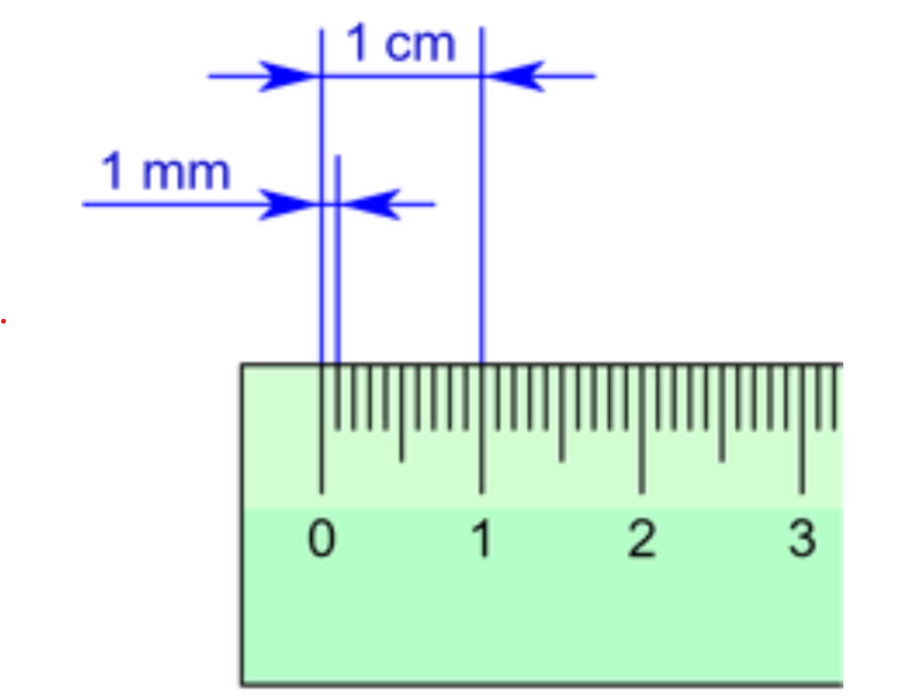
\includegraphics[scale=0.2]{../VATLY10-HK1-2025/figs/ss1}}
	
	\loigiai{
	\begin{itemchoice}
		\itemch Giá trị trung bình của phép đo này là $\bar{d} = \frac{d_1+d_2+d_3+d_4}{4} = \SI{2.4}{\centi\meter}$.
		\itemch Sai số tuyệt đối các lần đo
		\begin{align*}
			\Delta d_1 &= \bar{d} - d_1 = 0,1 \\
			\Delta d_2 &= \bar{d} - d_2 = 0 \\
			\Delta d_3 &= \bar{d} - d_3 = 0,1 \\
			\Delta d_4 &= \bar{d} - d_4 = 0
		\end{align*}
		Sai số tuyệt đối trung bình của 4 lần đo được
		$$ \overline{\Delta d} = \dfrac{\Delta d_1 + \Delta d_2 + \dots + \Delta d_4}{n} = \dfrac{0,1+0+0,1+0}{4} = \SI{0.05}{\centi\meter}$$ 
		\itemch Sai số tuyệt đối $\Delta d$ là $\Delta d = \overline{\Delta d} + \Delta d_{\text{dc}} = \SI{0.1}{\centi\meter}$.
		\itemch Kết quả đo: $d = \xsi{2,4\pm 0,1}{\centi\meter}$.
		\end{itemchoice}
	}
\end{ex}
\Closesolutionfile{ans}
\subsection{TRẢ LỜI NGẮN}
\setcounter{ex}{0}
\Opensolutionfile{ans}[ans/FINAL-CHAPTER1-SA]

%===========================================Trả lời ngắn
\begin{ex}
	Hãy xác định sai số dụng cụ của cây bút chì trong trường hợp dưới đây theo đơn vị centimet (\si{\centi\meter}):
\begin{center}
	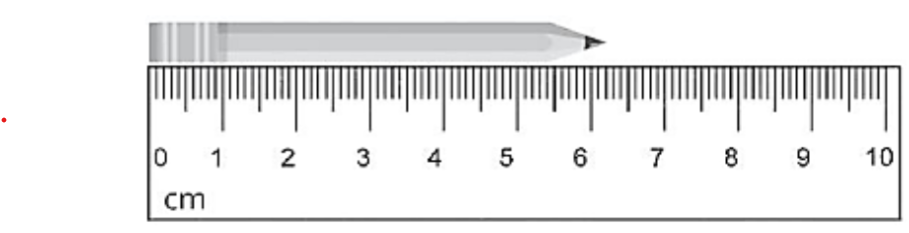
\includegraphics[scale=0.5]{figs/ss2}
\end{center}
	\shortans[oly]{0.05}
	\loigiai{Sai số dụng cụ bằng nửa độ chia nhỏ nhất: $\Delta x = \Delta x_{dc} = \dfrac{0,1}{2} = \SI{0.05}{\centi\meter}.$\\
		Kết quả đo: $x = \bar{x} \pm \Delta x = \xsi{6,20\pm0,05}{\centi\meter}.$	}
\end{ex}

\begin{ex}
	{Cạnh của một hình lập phương đo được là $a=\xsi{2.00\pm0.01}{\centi\meter}$. Sai số tuyệt đối của phép đo gián tiếp tính thể tích khối lập phương}
	\shortans[oly]{0.12}
	\loigiai{Thể tích của khối lập phương: $V = a^3 = (2,00)^3 = 8,00 \text{ cm}^3.$\\
	Sai số tỉ đối: $\dfrac{\Delta V}{V} = 3 \cdot \dfrac{\Delta a}{a} = 3 \cdot \dfrac{0,01}{2,00} = \SI{0.015}{\centi\meter^3}$\\
	Sai số tuyệt đối của phép đo: $\Delta V = 0,015V = 0,015 \cdot 8,00 = \SI{0.12}{\centi\meter^3}$.}
\end{ex}

\begin{ex}
	{Để tính gia tốc rơi tự do $g$, người ta có thể dùng công thức tính chu kì của một con lắc đơn gồm một vật nặng có kích thước nhỏ treo vào một dây nhẹ, không co giãn:
		$$ T = 2\pi\sqrt{\dfrac{\ell}{g}},$$
		trong đó, $T$ là thời gian để vật nặng thực hiện một dao động và $\ell$ là chiều dài sợi dây. Trong thí nghiệm với con lắc đơn, người ta đo được: $\ell =\xsi{0,350 \pm 0,005}{\meter}$ và $T =\xsi{1,18 \pm 0,02}{\second}$. Giá trị trung bình của gia tốc rơi tự do qua phép đo này là bao nhiêu $\si{\meter/\second^2}$? Lấy $\pi=3,14 \pm 0,01$}
	\shortans[oly]{9.92}
	\loigiai{Gia tốc rơi tự do: $g = 4\pi^2 \cdot \dfrac{\ell}{T^2} = 4\pi^2 \cdot \dfrac{0,350}{(1,18)^2} \approx \SI{9.92}{\meter/\second^2}$.}
\end{ex}


\begin{ex}
	Một người dùng bình chia độ (như hình) để đo thể tích của chất lỏng theo đơn vị \si{\centi\meter^3}. Kết quả phép đo là bao nhiêu?
	\begin{center}
		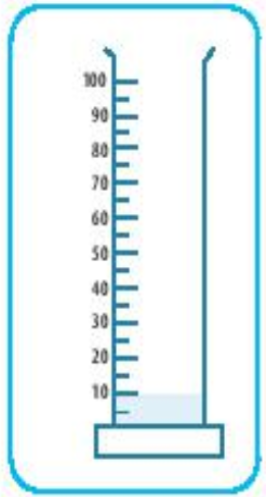
\includegraphics[scale=0.8]{figs/ss3}
	\end{center}
	\shortans[oly]{10,5}
	\loigiai{Quan sát mực nước trên bình chia ta thấy mực nước dừng lại ở vạch $\SI{10.5}{\centi\meter^3}$.}
\end{ex}
\Closesolutionfile{ans}
\subsection{TỰ LUẬN}
\setcounter{ex}{0}
\Opensolutionfile{ans}[ans/FINAL-CHAPTER1-TL]
\begin{ex}
	(1 điểm) Tìm số CSCN của các số sau:
	\begin{enumerate}[label=\alph*)]
		\item $78,9\pm 0,2$;
		\item $3,788\cdot10^9$;
		\item $2,46\cdot10^6$;
		\item $0,0053$.
	\end{enumerate}
	\loigiai{
		\begin{enumerate}[label=\alph*)]
			\item 3 CSCN;
			\item 4 CSCN;
			\item 3 CSCN;
			\item 2 CSCN.
		\end{enumerate}
	}
\end{ex}

\begin{ex}
	(1 điểm) Trong quá trình thực hành tại phòng thí nghiệm, một bạn học sinh vô tình làm vỡ nhiệt kế thuỷ ngân và làm thuỷ ngân đổ ra ngoài như Hình \ref{fig:2P-2}. Em hãy giúp bạn học sinh đó đưa ra cách xử lí thuỷ ngân đổ ra ngoài đúng cách để đảm bảo an toàn.
	\begin{center}
		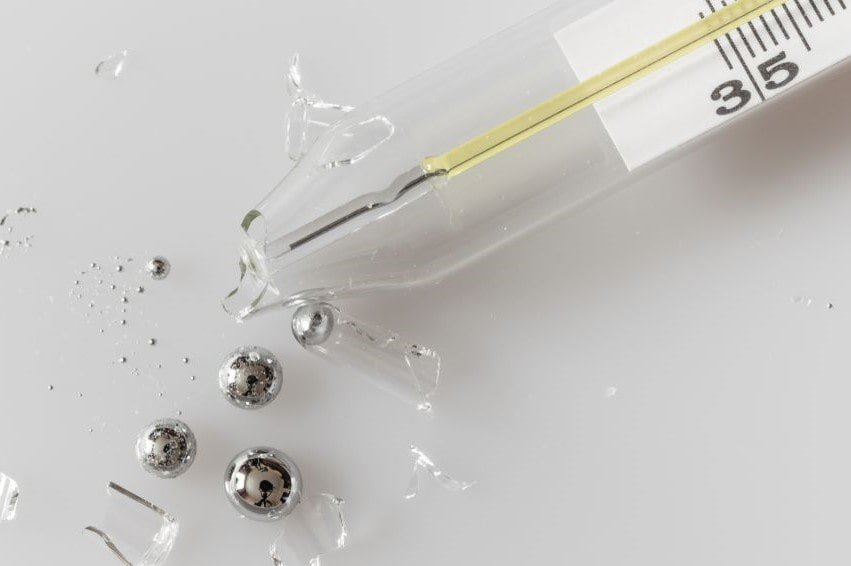
\includegraphics[width=0.3\linewidth]{figs/FINAL-CHAPTER1-2}
		\captionof{figure}{Thuỷ ngân bị đổ ra khỏi nhiệt kế}
		\label{fig:2P-2}
	\end{center}
	\loigiai{
		Cách xử lí đúng nguyên tắc an toàn: báo cho giáo viên tại phòng thí nghiệm, sơ tán các bạn học sinh ở khu vực gần đó, tắt quạt và đóng hết cửa sổ để tránh việc thuỷ ngân phát tán trong không khí. Người dọn dẹp phải sử dụng găng tay và khẩu trang để dọn sạch thuỷ ngân, tuyệt đối không được tiếp xúc với thuỷ ngân bằng tay trần.
	}
\end{ex}


\begin{ex}
	(1 điểm) Hai người cùng đo chiều dài của cánh cửa sổ, kết quả thu được như sau:
	\begin{itemize}
		\item Người thứ nhất: $d=\xsi{120\pm1}{\centi\meter}$;
		\item Người thứ hai: $d=\xsi{120\pm 2}{\centi\meter}$;
	\end{itemize}
	Trong hai người, ai là người đo chính xác hơn? Vì sao?
	\loigiai{
		Người 1 đo chính xác hơn vì với cùng một giá trị trung bình nhưng sai số tuyệt đối trong phép đo của người 1 bé hơn sai số tuyệt đối trong phép đo của người 2.\\
		Hoặc có thể tính sai số tỉ đối $\delta_1=\SI{0.83}{\percent}$ và $\delta_2=\SI{1.67}{\percent}$. Vì $\delta_1<\delta_2$ nên người 1 đo chính xác hơn.	
	}
\end{ex}

\Closesolutionfile{ans}